\chapter{Implementation}
In this chapter the implementation of the compiler will be explained.

\begin{figure}[!ht]
\centering
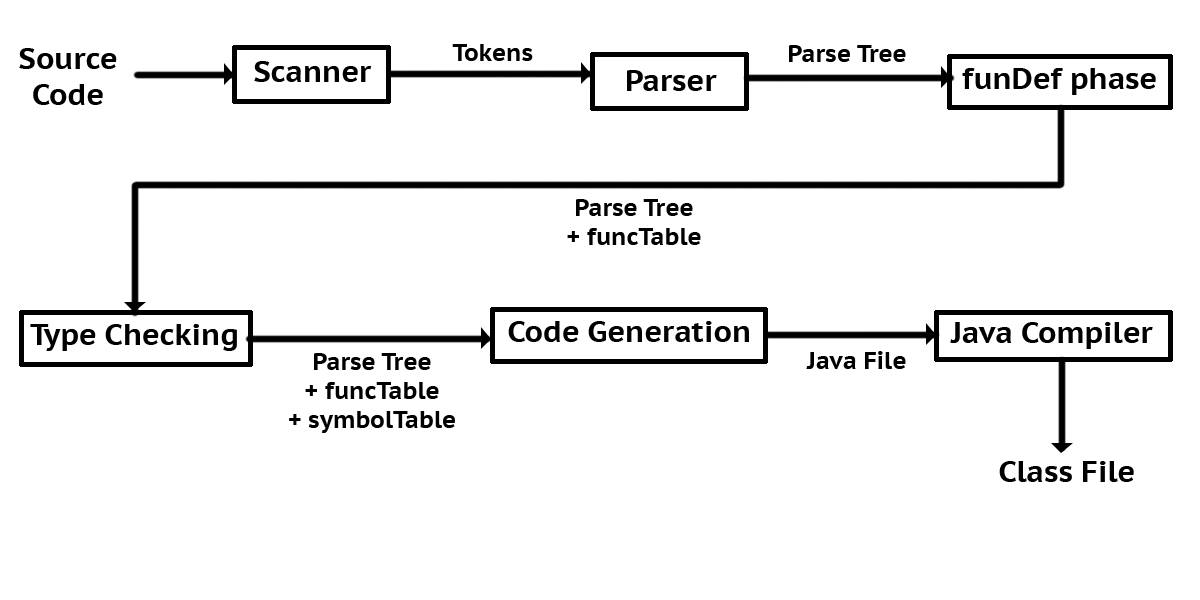
\includegraphics[scale=0.35]{billeder/compilerStructure}
\caption{Compiler structure}
\label{cs}
\end{figure}


The phases the compiler goes through are show in figure \ref{cs}. Before this though, the ANTLR tool has generated a scanner and a parser using the grammar showed in section 4.2. The ANTLR scanner is used to transform the source code into tokens. These tokens are then used by the ANTLR parser to generate the parsetree. After this the compiler does 3 triversals of this parsetree. First triversal is the funcDef phase, where every function the user has written is added to a funcTable for use in later phases. Second triversal is the Type checking phase. This phase uses a symboltable to check that the type and scope rules are followed by the code. The third triversal is the code generation phase, where the compiler goes through the parse tree and translates it to java code. Lastly the java code is sendt to the javac compiler and compiled to the finnished java robot class usable by robocode.


\section{ANTLR}
The ANTLR tool takes as input the sourcecode the user wants to parse along with the grammar for the language. It then does the lexical analysis to scan the sourcecode for compliance with the grammar to create the tokens, and after that it parses the sourcecode to create a parse tree. On top of creating the parse tree, the ANTLR tool generates 2 visitor patterns, which can be extended and used. The first and simplest is the listener. The listener has 2 functions for each node in the parse tree, one called enter and one called exit. With the listener a walker is needed to triverse the parse tree. As the walker visits nodes in the parse tree it calls the right function in the listener. The enter function is called as soon as the walker visits the node. After this the walker visits any child nodes. When it returns from these child notes the exit function is called. The second visitor pattern is the visitor. The visitor has one function per node. Each node function is responsible for calling all child node functions it has. This gives the coder more freedom in when to call the child nodes and i which order. Also the visitor supports return types on the functions, which makes it possible to pass data from one node to the caller node. 


\section{Function definition}
After ANTLR has produced the parse tree, base listener and base visitor, the function definition phase starts. In this phase every function that already exists in Robocode, will be mapped to the names defined in the appendix,(Indsæt reference til apendix her!!!!!) and added to the function table. Also every user defined function or actions will be added to this function table. 

\subsection{FuncSymbol \& FuncSymbolTable}
To keep track of the varies functions and their parameters, return values and Robocode names, a FuncSymbol class is used as representation for a single function and a FuncSymbolTable class is used to keep track of every FuncSymbol in the program.
The FuncSymbol has a string properties for Name, Type, ReturnType, original Robocode names and a string array for the parameters.

The FuncSymbolTable is basically a key/value pair HashMap. Where the key is the type of the function followed by the name of the function. The type in this case, can be either Function or Action from user defined functions, Tank, Gun, Battlefield, Radar or Utils from Robocode functions or the name of the event from Robocode events.
This class has two functions, GetFuncSymbol and EnterFuncSymbol which can be found in listing \ref{FST}. 

The GetFuncSymbol takes a type and a name from a function, combines them, looks for them in the HashMap and returns the result.

EnterFuncSymbol takes a FuncSymbol and tries to add it to the HashMap. First it checks if a function with same type and name was already declared, if such a function exists, an error is thrown, otherwise the function is added to the HashMap.

\begin{lstlisting}[caption={FuncSymbolTable}, label={FST}]
public class FuncSymbolTable {

	public LinkedHashMap<String, FuncSymbol> Map = new LinkedHashMap<String, FuncSymbol>();

	public FuncSymbol GetFuncSymbol(String type, String name){
    	FuncSymbol sym = Map.get(type + name);
    	return sym;
	}

	public void EnterFuncSymbol(FuncSymbol fs){
    	FuncSymbol oldSym = GetFuncSymbol(fs.Type, fs.Name);
    	if (oldSym != null) {
        	Error e = new Error("Function already declared");
        	throw e;
    	}
    	Map.put(fs.Type + fs.Name, fs);
	}
}
\end{lstlisting}

Forklar måden hvor på vi mapper robocode funktioner til vores funktioner
Forklar om den listener og walker vi bruger og hvordan de virker. (I hvert fald  få forklaret hvodan vi implementere dem her, hvis de er beskrevet  i den section før)
Error handling
Forklar om de to forskellige functables der bliver generete af henholdsvis bruger og fra den fil der bilver loadet ind. 

\subsection{Robocode functions \& events}
To allow the type checker and code generation phase to do their jobs, every Robocode function and event needs to be added to the FuncSymbolTable. To do this a simple text file was created which line for line have each function written out in a specific manner. 

WE COULD EXPLAIN THE TEXTFILE AND THE ALGORITHM USED TO LOAD IT IN IF WE HAVE TIME!!

\subsection{Userdefined functions \& actions}
To load the user defined functions from the program, a traverse of the parse tree is done using the ANTLR generated walker/listener. For every Function and Action the listener visits, a new FuncSymbol is created and added to the FuncSymbolTable. This is done with the FuncListener class, which extends the BaseListener ANTLR created.
 
The FuncListener class overrides the Enter/Exit Action declaration functions, the Enter/Exit Function declaration functions and the Enter parameter function. In the Enter Action and Function declaration functions, a new FuncSymbol is created called CurrentFunc. To CurrentFunc a name and a type is added, and in the Function case a return type is added as well. Name, type and return type are found using the parse tree.
In the Enter parameter function adds a new parameter to the CurrentFunc's array of parameters. 
Now in the Exit Action and Function declaration functions the CurrentFunc gets added to the FuncSymbolTable. 
The reason the CurrentFunc is added in the Exit functions, is that the walker have to visit all the parameters. 

\section{Type checking} 
After the first traversal of the parse tree using the FuncListener, every function is now defined in the function table and we can begin type checking. To do type checking a Symbol- and a SymbolTable class are used to keep track of every variable and their scope, using these two classes the SymbolTypeVisitor class checks for type compatibility. 

\subsection{Symbol \& symbol table}
Every variable in the program is represented by the Symbol class. The Symbol class has the properties String Name and Type, Symbol Var and int Depth. The Name and Type represents the name and type of the variable, the interesting parts is the Var and Depth properties. Var is a reference to a Symbol of the same name but in a higher scope, this would work as stack for all symbols of the same name, where the top of the stack will be the most inner scope and therefore the one used. The Depth property indicates the depth of the scope the symbol is in, with 0 being the global scope. 

The SymbolTable is mainly two things, the Map associates a name of a variable with a symbol as key value pairs, these symbols are the ones on top of the stack describes in the paragraph before. The scope is an array of arrays of symbols. Each index of the outer array is a scope and each inner array contains the symbols of that scope. 

The SymbolTable class has four functions: OpenScope, CloseScope, GetSymbol and EnterSymbol. 

OpenScope in listing \ref{OS} is used to open a new scope. Depth is a global variable, which keeps track of the current scope's depth. When OpenScope is run, the depth is incremented. If the Scope size is less than the depth + 1, a new array is added to the scope, otherwise the old array is cleared.

\begin{lstlisting}[caption={OpenScope function}, label={OS}]
public void OpenScope(){
    depth++;
    if (Scope.size() < depth+1){
        Scope.add(new ArrayList<Symbol>());
    }else {
        Scope.get(depth).clear();
    }
}
\end{lstlisting}

 The EnterSymbol function in listing \ref{ES}, is used to enter e new symbol into the SymbolTable. When EnterSymbol is run it firstly checks if there already exists a symbol with the same name, if this is the case it checks whether the depth of this symbol is the same depth as current scope. If the depths are the same, an error is thrown, since there can't exist two variables with the same name in the same scope. If no symbol exists in the Map or it is at another depth, a new symbol is created. This symbol gets the current depth in its depth property and it sets its var property to the old symbol. It then either replaces the new symbol with the old symbol or just adds it if the old symbol was null. 

The GetSymbol function looks up a symbol in the map and will return the name of that symbol.

\begin{lstlisting}[caption={EnterSymbol function}, label={ES}]
public void EnterSymbol(String name, String type){
    Symbol oldsym = Map.get(name);
    if (oldsym != null && oldsym.Depth == depth){
        Error e = new Error("Duplicate declaration of " + name);
        throw e;
    }else{
        Symbol newSym = new Symbol();
        newSym.Name = name;
        newSym.Type = type;
        newSym.Depth = depth;
        newSym.Var = oldsym;
        Scope.get(depth).add(newSym);
        Map.put(newSym.Name, newSym);
    }
}
\end{lstlisting}

CloseScope in listing \ref{CS}, is used to close the current scope. This is done by going through each symbol \textbf{s} at the current depth, and replacing \textbf{s} in the Map with \textbf{s.Var} which is a symbol with the same name but in a higher scope. If no such symbol exists, \textbf{s} is replaced with a null value. 

\begin{lstlisting}[caption={CloseScope function}, label={CS}]
public void CloseScope(){
    Scope.get(depth).forEach(s -> {
        Symbol prevSym = s.Var;
        Map.replace(s.Name, s, prevSym);
    });
    depth--;
}
\end{lstlisting}



\subsection{The SymbolTypeVisitor class}
The SymbolTypeVisitor class extends the BaseVisitor class from ANTLR and is the second traversal through the parse tree. It visits every single node in  the parse tree and each node return its type to the caller. At each node it is determined whether the types returned match with the expected type, errors are thrown if they don't match.

At the basic level the types are returned as they are, which is the functions visitNum, visitString and visitBool, that can be found in listing \ref{VT}.

\begin{lstlisting}[caption={SymbolTypeVisitor - visitNum, visitString and visitBool functions}, label={VT}]
@Override
public String visitNum(GrammarParser.NumContext ctx) {
    return "Num";
}

@Override
public String visitString(GrammarParser.StringContext ctx) {
    return "String";
}

@Override
public String visitBool(GrammarParser.BoolContext ctx) {
    return "Bool";
}
\end{lstlisting}

Also at the basic level variable ids are looked up in the SymbolTable and their type is returned, an error is thrown if the variable isn't found in the SymbolTable, as shown in listing \ref{VID}.

\begin{lstlisting}[caption={SymbolTypeVisitor - visitId function}, label={VID}]
@Override
public String visitId(GrammarParser.IdContext ctx) {
    String test = ctx.getText();
    Symbol sym = ST.GetSymbol(ctx.getText());
    if (sym == null){
        Error e = new Error("Error at line: " +
                ctx.start.getLine() + ": Variable not found");
        throw e;
    }
    return sym.Type;
}
\end{lstlisting}

When visiting and, or, minus, not, mul, rel and eq expressions each expression type is calculated and compared to what is expected. Afterwards either an error is thrown or the right type is returned. An example of such function is the or-expression, which can be found in listing \ref{VOR}.

\begin{lstlisting}[caption={SymbolTypeVisitor - visitOrexpr function}, label={VOR}]
@Override
public String visitOrexpr(GrammarParser.OrexprContext ctx) {
    String left = visit(ctx.expr(0));
    String right = visit(ctx.expr(1));
    if (left.equals("Bool") && right.equals("Bool")){
        return "Bool";
    }else{
        Error e = new Error("Error at line: " +
                ctx.start.getLine() + ": Expression did not evaluate to Bool.");
        throw e;
    }
}
\end{lstlisting}

The add-expression in listing \ref{VADD}, is a bit special as the plus operator can be used on two numbers or a string and any other type. Therefore the function checks if both expressions evaluate to a number, or one of them is a string and the operator is a plus, it throws an error if none of the above is true else it returns the appropriate type. 

\begin{lstlisting}[caption={SymbolTypeVisitor - visitAddexpr function}, label={VADD}]
@Override
public String visitAddexpr(GrammarParser.AddexprContext ctx) {
    String left = visit(ctx.expr(0));
    String right = visit(ctx.expr(1));
    if (left.equals("Num") && right.equals("Num")) {
        return "Num";
    }else if((left.equals("String") || right.equals("String")) && ctx.op.getText().equals("+") ) {
        return "String";
    }else{
        Error e = new Error("Error at line: " +
                ctx.start.getLine() + ": Expression types did not match.");
        throw e;
    }
}
\end{lstlisting}

The function visitAssign in listing \ref{VAS}, checks whether the type of the symbol found from the id = the expression's type. It throws errors if the id doesn't match any symbols or the types don't match. 

\begin{lstlisting}[caption={SymbolTypeVisitor - visitAssign function}, label={VAS}]
@Override
public String visitAssign(GrammarParser.AssignContext ctx) {
    String id = ctx.ID().getText();
    Symbol sym = ST.GetSymbol(id);
    if (sym == null){
        Error e = new Error("variable not found");
        throw e;
    }
    if (!sym.Type.equals(visit(ctx.expr()))){
        Error e = new Error("Error at line: " +
                ctx.expr().start.getLine() + ": Expression and variable are not type compatible");
        throw e;
    }
    return sym.Type;
}
\end{lstlisting}

The function visitVardcl in listing \ref{VAD}, enters a new symbol in the SymbolTable. The type is found at the variable declaration Node or at the assign node. visitVardcl determines where to find the id and adds the new symbol to the SymbolTable. 

\begin{lstlisting}[caption={SymbolTypeVisitor - visitVardcl function}, label={VAD}]
@Override
public String visitVardcl(GrammarParser.VardclContext ctx) {
    if (ctx.getChild(1) instanceof GrammarParser.AssignContext){
        ST.EnterSymbol(((GrammarParser.AssignContext) ctx.getChild(1)).ID().getText(), ctx.TYPE().getText());
        visit(ctx.assign());
    }else {
        ST.EnterSymbol(ctx.ID().getText(), ctx.TYPE().getText());
    }
    return ctx.TYPE().getText();
}
\end{lstlisting}

The visitBlock function in listing \ref{VB}, opens a new scope and if its parent is the Action declaration, any parameter of the Action declaration  is added to the scope. The function then visits all the statements in the block and then closes the scope. 

\begin{lstlisting}[caption={SymbolTypeVisitor - visitBlock function}, label={VB}]
@Override
public String visitBlock(GrammarParser.BlockContext ctx) {
    ST.OpenScope();
    if (ctx.parent instanceof GrammarParser.ActdclContext){
        FuncSymbol fs = FST.GetFuncSymbol("Action", ((GrammarParser.ActdclContext) ctx.parent).ID().getText());
        fs.Params.forEach(tuple -> {
            ST.EnterSymbol(tuple.x, tuple.y);
        });
    }
    visit(ctx.stmts());
    ST.CloseScope();
    return "null";
}
\end{lstlisting}

The function visitArgs in listing \ref{VAF} at line 1-8, visits each expression and concatenates with a comma in between and returns the whole thing as a string. 

visitFcall which is also found in listing \ref{VAF} at line 10-37, gets a function symbol from the FuncSymbolTable and then matches each argument type from the visitArgs with each parameter type in the function symbol. Errors are thrown if these don't match or the function id doesn't match any function in the FuncSymbolTable. visitAcall, visitUtilscall, visitBattlefieldcall, visitRadarcall, visitGuncall and visitTankcall functions works similarly to the visitFcall function.

\begin{lstlisting}[caption={SymbolTypeVisitor - visitArgs and visitFcall functions}, label={VAF}]
@Override
public String visitArgs(GrammarParser.ArgsContext ctx) {
    String result = visit(ctx.expr(0));
    for (int i = 1; i < ctx.expr().size(); i++){
        result = result + ", " + visit(ctx.expr(i));
    }
    return result;
}

@Override
public String visitFcall(GrammarParser.FcallContext ctx) {
    FuncSymbol fsym = FST.GetFuncSymbol("Function", ctx.ID().getText());
    if (fsym == null){
        Error e = new Error("Error at line: " +
                ctx.start.getLine() + ": Function not found");
        throw e;
    }
    if (!fsym.Type.equals("Function")){
        Error e = new Error("Error at line: " +
                ctx.start.getLine() + ": Incorrect function type.");
        throw e;
    }
    if(ctx.getChildCount() == 4) {
        String[] args = visit(ctx.args()).split(", ");
        for (int i = 0; i < args.length; i++) {
            String paramType = fsym.Params.get(i).y;
            String arg = args[i];
            if (!paramType.equals(arg)) {
                Error e = new Error("Error at line: " +
                        ctx.args().expr(i).start.getLine() +
                        ": Parameter number " + i + " not matched. Expected " + paramType);
                throw e;
            }
        }
    }
    return fsym.ReturnType;
}
\end{lstlisting}

visitEcall in listing \ref{VE}, is a bit special compared to the other call function, as it needs to check whether the function called is comparable with the event that it is called within. To do this, it checks the parent to see if that is an event declaration, if it is not, it checks the parent of the parent and so on, until it either reaches the event declaration or the root of the tree, if the root is reached an error is then thrown. If an event declaration is reached, the event declaration id and the event call id is used to look up the function in the FuncSymbolTable, if none is returned an error is thrown, otherwise the arguments are matched with the parameters as before, if successful the function's return type is returned. 

\begin{lstlisting}[caption={SymbolTypeVisitor - visitEcall function}, label={VE}]
@Override
public String visitEcall(GrammarParser.EcallContext ctx) {
    RuleContext parent = ctx.parent;
    while(parent != null){
        if(parent instanceof GrammarParser.EventdclContext){
            FuncSymbol fsym = RoboFST.GetFuncSymbol(((GrammarParser.EventdclContext) parent).ID().getText(), ctx.ID().getText());
            if (fsym == null){
                Error e = new Error("Error at line: " +
                        ctx.start.getLine() + ": Function not found");
                throw e;
            }
            if(ctx.getChildCount() == 5) {
                String[] args = visit(ctx.args()).split(", ");
                for (int i = 0; i < args.length; i++) {
                    String paramType = fsym.Params.get(i).y;
                    String arg = args[i];
                    if (!paramType.equals(arg)) {
                        Error e = new Error("Error at line: " +
                                ctx.args().expr(i).start.getLine() +
                                ": Parameter number " + i + " not matched. Expected " + paramType);
                        throw e;
                    }
                }
            }
            return fsym.ReturnType;
        }
        parent = parent.parent;
    }
    Error e = new Error("Event calls must be inside an event/when function");
    throw e;
}
\end{lstlisting}

visitDcls makes sure that the program the user wrote has one and only one Tankname, Repeatblock and Setupblock declared. 

\begin{lstlisting}[caption={SymbolTypeVisitor - visitDcls function}, label={VD}]
@Override
public String visitDcls(GrammarParser.DclsContext ctx) {
    if (ctx.tankname().size() < 1){
        Error e = new Error("A Tankname needs to be declared");
        throw e;
    }else if (ctx.tankname().size() > 1){
        Error e = new Error("Error at line: " +
                ctx.tankname(1).start.getLine() + ": Too many tank names.");
        throw e;
    }
    if (ctx.repeatblock().size() < 1){
        Error e = new Error("A Repeat block needs to be declared");
        throw e;
    }else if (ctx.repeatblock().size() > 1){
        Error e = new Error("Error at line: " +
                ctx.repeatblock(1).start.getLine() + ": Too many repeat blocks.");
        throw e;
    }
    if (ctx.setupblock().size() < 1){
        Error e = new Error("A Setup block needs to be declared");
        throw e;
    }else if (ctx.setupblock().size() > 1){
        Error e = new Error("Error at line: " +
                ctx.setupblock(1).start.getLine() + ": Too many setup blocks.");
        throw e;
    }
    super.visitDcls(ctx);
    return "null";
}
\end{lstlisting}



Forklar vi "overskriver" visitoren, eller vi bruger visitoren.
\section{Code generation}
The CodeGen class extends the BaseListener class and is the third and last traversal of the parse tree. At this point the program is type checked and ready to get translated into Java code, the CodeGen class generates a string containing the translated code. 

When visiting the literals bool, num and string nothing is changed and the text is returned. When visiting id an "\_" is added in front of the id, to make sure the id name doesn't clash with Java keywords. The literals id and num can be seen in listing \ref{VIM}. 

\begin{lstlisting}[caption={CodeGen - visitId \& visitNum functions}, label={VIM}]
@Override
public String visitId(GrammarParser.IdContext ctx) {
    return "_" + ctx.ID().getText();
}

@Override
public String visitNum(GrammarParser.NumContext ctx) {
    return ctx.NUM().getText();
}
\end{lstlisting}

When visiting expressions the only thing needed is to change AND, OR, IS=, NOT= and NOT is changed to their equivalent operator in Java. 

In the visitEcall function in listing \ref{VEC} the appropriate FuncSymbol is found in the FuncSymbolTable using the same method as the SymbolTypeVisitor class. visitEcall adds "e." in front of the function name, before it returns. The "e" will be the parameter of the event which this call is within. 

\begin{lstlisting}[caption={CodeGen - visitEcall function}, label={VEC}]
@Override
public String visitEcall(GrammarParser.EcallContext ctx) {
    FuncSymbol fsym;
    RuleContext parent = ctx.parent;
    while(parent != null){
        if(parent instanceof GrammarParser.EventdclContext){
            fsym = RoboFST.GetFuncSymbol(((GrammarParser.EventdclContext) parent).ID().getText(), ctx.ID().getText());
            if(ctx.getChildCount() == 5) {
                return "e." + fsym.RoboCodeName + "(" + visit(ctx.args()) + ")";
            }else {
                return "e." + fsym.RoboCodeName + "()";
            }
        }
        parent = parent.parent;
    }
    Error e = new Error("codeGen Error");
    throw e;
}
\end{lstlisting}

In all other Robocode calls, like the visitTankcall function found in listing \ref{VTC}, the appropriate FuncSymbol is found in the FuncSymbolTable and the Robocode name is returned with potential arguments.

\begin{lstlisting}[caption={CodeGen - visitTankcall function}, label={VTC}]
@Override
public String visitTankcall(GrammarParser.TankcallContext ctx) {
    FuncSymbol fs = RoboFST.GetFuncSymbol("Tank", ctx.ID().getText());
    if(ctx.getChildCount() == 5) {
        return fs.RoboCodeName + "(" + visit(ctx.args()) + ")";
    }else {
        return fs.RoboCodeName + "()";
    }
}
\end{lstlisting}

In Function and Action calls an "\_" are added in front of the id and potential parameters before returning. This is done like with the num, string and bool literals, so the id's don't clash with any Java keywords. Listing \ref{VFC} shows the visitFcall function.

\begin{lstlisting}[caption={CodeGen - visitFcall function}, label={VFC}]
@Override
public String visitFcall(GrammarParser.FcallContext ctx) {
    if (ctx.getChildCount() == 4){
        return "_" + ctx.ID().getText() + "(" + visit(ctx.args()) + ")";
    }else{
        return "_" + ctx.ID().getText() + "()";
    }
}
\end{lstlisting}

The visitIfstmt function uses a StringBuilder to add the \textbf{if} followed by any \textbf{elseif} if needed, at the end the StringBuilder returns as a string. The visitIfstmt function is shown in listing \ref{VISTM}

\begin{lstlisting}[caption={CodeGen - visitIfstmt function}, label={VISTM}]
@Override
public String visitIfstmt(GrammarParser.IfstmtContext ctx) {
    StringBuilder buf = new StringBuilder();
    buf.append("if(");
    buf.append(visit(ctx.expr()));
    buf.append(")");
    buf.append(visit(ctx.block(0)));
    for(int i = 0; i< ctx.elseif().size(); i++){
        buf.append(visit(ctx.elseif(i)));
    }
    if (ctx.block().size() > 1){
        buf.append("else");
        buf.append(visit(ctx.block(1)));
    }
    return buf.toString();
}
\end{lstlisting}

The visitVardcl function shown in listing \ref{VVDCL}, changes the type declared in the program to the equivalent type in Java. String and Bool will be changes to string and boolen, where the type Num will be changed to a double. Another thing worth mentioning is the "\_" in front of the ids, for the same reasons as mentioned before.

\begin{lstlisting}[caption={CodeGen - visitVardcl function}, label={VVDCL}]
@Override
public String visitVardcl(GrammarParser.VardclContext ctx) {
    String result;
    if (ctx.TYPE().getText().equals("Num")){
        result = "double ";
    }else if(ctx.TYPE().getText().equals("Bool")){
        result = "boolean ";
    }else{
        result = "String ";
    }
    if (ctx.getChild(1) instanceof GrammarParser.AssignContext){
        result += visit(ctx.assign());
    }else {
        result += "_" + ctx.ID().getText() + ctx.SEMI().getText() + "\n";
    }
    return result;
}
\end{lstlisting}

The visitEventdcl function in listing \ref{VEDCL} is worth noting the added "on"  and the added "Event", these are used to create the Robocode eventhandler and the Robocode event. The "e" added after "Event" corresponds to the e in visitEcall.

\begin{lstlisting}[caption={CodeGen - visitEventdcl function}, label={VEDCL}]
@Override
public String visitEventdcl(GrammarParser.EventdclContext ctx) {
    String id = StringUtils.capitalize(ctx.ID().getText());
    return "public void on" + id + "( " + id + "Event e )" + visit(ctx.block());
}
\end{lstlisting}

In the visitFuncdcl function  a new public Java function is created with the return type with the appropriate return type, name, block and possibly parameters. Once again an "\_" is added in front of the id, for the same reasons as before.

\begin{lstlisting}[caption={CodeGen - visitFuncdcl function}, label={VFDCL}]
@Override
public String visitFuncdcl(GrammarParser.FuncdclContext ctx) {
    String type;
    if (ctx.TYPE().getText().equals("Num")){
        type = "double ";
    }else if(ctx.TYPE().getText().equals("Bool")){
        type = "boolean ";
    }else{
        type = "String ";
    }
    if (ctx.getChildCount() == 8) {
        return "public " + type + " _" + ctx.ID().getText() + "(" + visit(ctx.params()) + ")" + visit(ctx.functionBlock());
    }else{
        return "public " + type + " _" + ctx.ID().getText() + "()" + visit(ctx.functionBlock());
    }
}
\end{lstlisting}

The visitSetupblock and visitRepeatblock functions shown in listing \ref{VSRB} are a bit special as the Repeat block(is the while(true) statement in the Run function in Java) is inside the Setup block(Run function) in Java. To do this Setup block creates the void function and adds the block, then cuts of the last curly bracket adds the Repeat block, which is renamed to while(true) and puts back the curly bracket. 

\begin{lstlisting}[caption={CodeGen - visitSetupblock \& visitRepeatblock functions}, label={VSRB}]
@Override
public String visitSetupblock(GrammarParser.SetupblockContext ctx) {
    String result = "public void run()" + visit(ctx.block());
    result = result.substring(0, result.length()-2);
    return result + visit(((GrammarParser.DclsContext) ctx.parent).repeatblock(0)) + "}";
}

@Override
public String visitRepeatblock(GrammarParser.RepeatblockContext ctx) {
    return "while (true)" + visit(ctx.block());
}
\end{lstlisting}

In the visitProg function a StringBuilder is used to add the import statements needed for Java to be able to compile the program. After that the class is declared using the Tankname and then extends Robot to the class declaration. After this the entire program is added followed by a closing curly bracket. The code generation is now complete and a string with the entire program in Java code is returned. 

\begin{lstlisting}[caption={CodeGen - visitProg function}, label={VP}]
@Override
public String visitProg(GrammarParser.ProgContext ctx) {
    StringBuilder buf = new StringBuilder();
    buf.append("import robocode.*;\n");
    buf.append("import static robocode.util.Utils.*;\n");
    buf.append("public class ");
    buf.append(StringUtils.capitalize(visit(ctx.dcls().tankname(0))));
    buf.append(" extends Robot {\n ");
    buf.append(visit(ctx.dcls()));
    buf.append("}");
    System.out.print(buf.toString());
    return buf.toString();
}
\end{lstlisting}


TO DO
Rename Txt og TEXT til String.
Open og close scope i functionBlockContext
CodeGen errors
Ændre while i codegen
Lav billede til Environment store model, og forklar det!
Apendix, skriv tekst til det vi har, overvej om der skal tilføjes kode eksempler.
Formuler en problem stilling i introduction.


